\documentclass[a4paper,12pt,twoside,fleqn]{book}

\usepackage{amssymb}
\usepackage{amsmath}
\usepackage{unicode-math}
\usepackage{seqsplit}

\usepackage[a4paper,top=.5in,bottom=.5in,left=.5in,right=.5in]{geometry}
\usepackage{booktabs}
\usepackage[svgnames]{xcolor}
\usepackage{pdfpages}
\usepackage{minted}
\usepackage[skins,minted]{tcolorbox}
\usepackage{csquotes}
\usepackage{fancyhdr}
\usepackage{titlesec}
\usepackage{titling}
\usepackage[hidelinks,hyperfootnotes=false,breaklinks=true,pdfauthor={Winterer, Mathis Aaron},pdftitle={Bedeutung von starken Primzahlen für die heutige Zeit},pdfsubject={Mathematische Exemplifikation des RSA-Algorithmuses},pdfkeywords={RSA,Verschlüsselung,Kryptographie,Mathematik,Primzahlen},colorlinks=true,linkcolor=black,filecolor=magenta,urlcolor=red,citecolor=blue]{hyperref}
\usepackage{tocloft}
\usepackage{fontspec}
\usepackage{polyglossia}
\usepackage[backend=biber,bibstyle=authoryear,style=alphabetic,seconds=true,]{biblatex}

\setmainlanguage[variant=german,spelling=new,capitaleszett=true,babelshorthands=true]{german}
\setmainfont{IBM Plex Mono}
\setsansfont{IBM Plex Mono}
\setmonofont{IBM Plex Mono}
\setmathfont{STIX Two Math}

\emergencystretch=1em

\graphicspath{{figs/}}
\addbibresource{bib.bib}
\definecolor{mintbg}{rgb}{0.23, 0.27, 0.29}
\definecolor{red}{HTML}{FF6961}
\usemintedstyle[csharp]{github-dark}
\setminted[csharp]{
  mathescape,
  frame=leftline,
  framesep=2mm,
  numberblanklines,
  numbersep=12pt,
  numbersep=5pt,
  baselinestretch=1.2,
  rulecolor=red,
  stripall,
  tabsize=4,
  funcnamehighlighting=true,
  autogobble,
  linenos,
  fontsize=\footnotesize,
  bgcolor=mintbg,
  breaklines,
}
\newtcblisting{cminted}[2][]{listing engine=minted, listing only,#1, title=#2, minted language=csharp, colback=mintbg}

\titleformat{\chapter}[block]{\huge\bfseries}{\thechapter.}{0.5em}{}[\titlerule\titlerule\vspace{-2em}]

\fancypagestyle{plain}{%
  \lhead{}
  \fancyhead[LO]{}
  \fancyhead[RE]{}
  \fancyhead[LE,RO]{}
  \renewcommand{\headrulewidth}{0pt}
  \fancyfoot{}
  \fancyfoot[LO]{}
  \fancyfoot[RE]{}
  \fancyfoot[LO,RE]{\thepage}
  \renewcommand{\footrulewidth}{1pt}
}

\futurelet\TMPfootrule\def\footrule{{\color{black!15}\TMPfootrule}}

\setlength{\cftsubsubsecnumwidth}{4.5em}
\renewcommand{\baselinestretch}{1.2} 
\setcounter{secnumdepth}{3}
\setcounter{tocdepth}{3}
\setlength{\parindent}{0pt}
\setlength{\footskip}{20pt}
\titlespacing*{\chapter}{0pt}{-19pt}{6em}
\renewcommand{\cfttoctitlefont}{\sffamily\bfseries\Large}
\renewcommand{\cftchapfont}{\bfseries}
\renewcommand{\cftsubsecfont}{\normalfont}
\renewcommand{\maketitle}{%
  \begin{center}
    \Huge\thetitle\\
    \vspace{1em}
    \normalsize\textit{Eine Einführung in das RSA-Verschlüsselungssystem}\\
    \vspace{2em}
    \Large\theauthor\\
    \vspace{2em}
    \large\textit{\textlang{german}{\today}}
  \end{center}
  \newpage
}

\title{Bedeutung von starken Primzahlen für die heutige Zeit}
\author{Winterer, Mathis Aaron}

\begin{document}
  \nonfrenchspacing
  \frontmatter{}
  \pagenumbering{gobble}
  \maketitle

  \pagestyle{plain}
  \pagenumbering{roman}
  \tableofcontents
  \newpage
  \listoffigures
  \newpage
  \listoftables
  \newpage

  \mainmatter{}
  \chapter{Einleitung}

Kryptographie und Verschlüsselungssysteme wurden schon im Antiken Rom verwendet um Nachrichten zu verschlüsseln\cite{aichner22}, doch heutzutage wären Verschlüsselungssysteme wie der \textquote{Cäsar-Chiffre} gegenüber eines Computers nutzlos.
Die Rolle von Kryptographie ist aufgrund des leichten Zugangs der Allgemeinheit zu leistungsstarken Computern, welche das Brechen von \textquote{schwachen} Verschlüsselungssystemen automatisiert und beschleunigt haben, um einiges angestiegen.
Aufgrund der nun verfügbaren Rechenleistung wurde die Notwendigkeit für stärkere Verschlüsselungssysteme immer größer. Zur Zeit verwendete Verschlüsselungssysteme sind so konzipiert, dass sie mathematisch schlecht rückwärts zu berechnen sind.
Hierzu werden standardmäßig große Primzahlen verwendet, da zur Zeit kein effizienter Algorithmus zur Berechnung von großen Primzahlfaktoren bekannt ist, welcher nicht die Verwendung eines Quantencomputers erfordern würde.
Das \textquote{brute-forcing} moderner Verschlüsselungssysteme ist so ineffizient, dass nur ein Teilschritt bis zu fünfzehnhundert Jahre dauern kann\cite{kleinjung10}.
\textquote{Für unsere Berechnungen waren mehr als $10^{20}$ Operationen erforderlich. Mit dem Äquivalent von fast 2000 Jahren Rechenzeit auf einem AMD Opteron mit einem Kern von 2,2 GHz [\ldots]}\cite{kleinjung10}.
Verschlüsselungssysteme sind aufgrund dieser hohen Anforderungen gegenüber der Resistenz gegen Angriffe äußerst komplexe Systeme welche in der Informationssicherheit eine entscheidende Rolle bei der Sicherung von sensiblen Daten sowohl in der Übertragung als auch bei der Speicherung spielen\cite{aichner22}.
Das Ziel dieser Facharbeit ist es den weit verbreiteten und etablierten RSA-Algorithmus zu Analysieren und zu Implementieren. Hierfür werden die einzelnen Teilschritte und verwendeten mathematischen Prinzipien und Funktionen erläutert und beispielhaft dargestellt sowie als Teil eines Programms in C\# implementiert, so dass die Funktionen der Schlüsselerzeugung, der Verschlüsselung, der Entschlüsselung und der Signierung verfügbar sind.
\newpage

\section{Hintergrund der RSA-Verschlüsselung}

$n-1=d\times{}2^j$

\begin{cminted}{MillerRabin.cs}
private static (BigInteger, BigInteger) FirstPart(BigInteger n)
{
    // nMinusOne
    BigInteger nMo = n - 1;
    BigInteger j = 0;
    BigInteger d = nMo;

    // Divide $n - 1$ By $2$ Until The Result Is Odd, Incrementing `$j$` Everytime And Storing The Result In `$d$`, So That `$n - 1 = d * 2^j$`
    while (d % 2 == 0)
    {
        d /= 2;
        j++;
    }

    return (d, j);
}
\end{cminted}
\newpage

\begin{figure}[ht]
  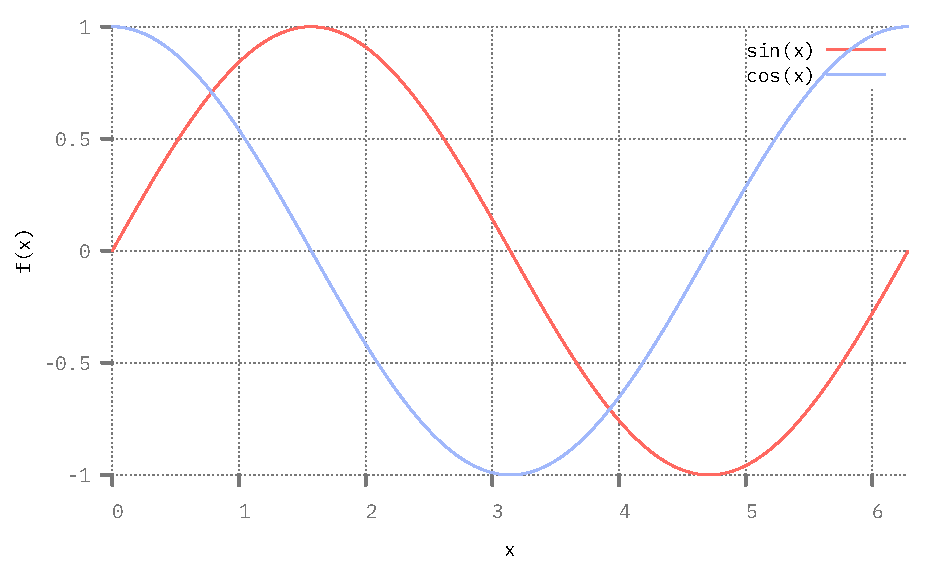
\includegraphics{sinx.pdf}
  \caption{sin(x) über [0; 6,28]}
\end{figure}

\begin{table}
  \center
\begin{tabular}{@{}llr@{}} \toprule
\multicolumn{2}{c}{Item} \\ \cmidrule(r){1-2}
Animal & Description & Price (\$)\\ \midrule
Gnat & per gram & 13.65 \\
& each & 0.01 \\
Gnu & stuffed & 92.50 \\
Emu & stuffed & 33.33 \\
Armadillo & frozen & 8.99 \\ \bottomrule
\end{tabular}
  \caption{Tabelle}
\end{table}

\newpage
\section{Anwendungsbereiche der RSA-Verschlüsselung}

  \newpage
  \chapter{Mathematische Grundlagen der RSA-Verschlüsselung}

% ✓Definition und ✓Anwendungsbeispiel + Wofür (Warum mit dieser Methode => Speed)
\section{Kleiner fermatscher Satz}

Der kleine fermatsche Satz, benannt nach seinem Entdecker Pierre de Fermat, ist ein Satz in der Zahlentheorie, welcher eine Kongruenz zwischen einer natürlichen Zahl $a$ und einer Primzahl $p$ herstellt.\cite{wa01}

Wenn $a$ eine beliebige natürliche Zahl, die nicht durch $p$ teilbar ist, und $p$ eine beliebige Primzahl seien, dann gilt:

\begin{equation}
  \begin{split}
    &\left\{\,p \in \mathbb{P}\, \right\}\\
    &\left\{\,a \in \mathbb{N}\mid ggT(a,p) = 1\, \right\}\\
    &a^{p} \equiv a \pmod{p}\\
  \end{split}
\end{equation}

Dies bedeutet, dass der Rest bei der Division von $a^{p}$ durch $p$ immer $a$ ist:

\begin{equation}
  \begin{split}
    &2^{3} \equiv 2\pmod{3}\\
    &4^{17} \equiv 4\pmod{17}\\
    &5^{7} \equiv 5\pmod{7}\\
  \end{split}
\end{equation}

Es finden sich in verschiedenen Quellen\cite{wa01}\cite{mw01} auch leicht abgeänderte Formeln wie:

\begin{equation}
  \begin{split}
    &(a^{p-1}-1) \bmod p = 0\\
    &a^{p-1} \equiv 1\pmod{p}
  \end{split}
\end{equation}

Für meine Zwecke verwende ich die als drittes beschriebene $a^{p-1} \equiv 1\pmod{p}$ Formel, da die erste und zweite Formel keinen Mehrwert bei meiner Anwendung bieten.

\newpage

\section{Primzahltests}
Der Miller-Rabin-Test ist ein probalistischer Primzahltest, dies bedeutet, dass der Algorithmus nicht immer zweifelsfrei korrekte Ergebnisse berechnet, jedoch kann die Genauigkeit der Ergenisse durch mehrfaches Durchlaufen des Algorithmus verbessert werden.
Der Miller-Rabin-Test hat für eine Iteration eine Wahrscheinlichtkeit kleiner als $\frac{1}{4}$ eine zusammengesetze Zahl als Primzahl zu erkennen. Aufgrund dessen ist es empfehlenswert den Algorithmus über mehrere Iterationen auszuführee, sodass die Wahrscheinlichtkeit des Fehlers vernachlässigbar wird.
Nach $i$ Iterationen ist die Wahrscheinlichtkeit des Fehlers $(\frac{1}{4})^i$. Somit ist sie für $10$ Iterationen schon rund $0.00000095367431640625$, was für die Primzahlselektion des RSA-Algorithmus ausreichend ist. Abbildung \ref{mr_error} zeigt den Verlauf der Fehlerwahrscheinlichkeit von $1$ bis $100$ Iterationen und illustriert deutlich, dass der Miller-Rabin-Test mit wenigen Iterationen einen ausreichend präziser Primzahltest bietet.

\begin{figure}[ht]
  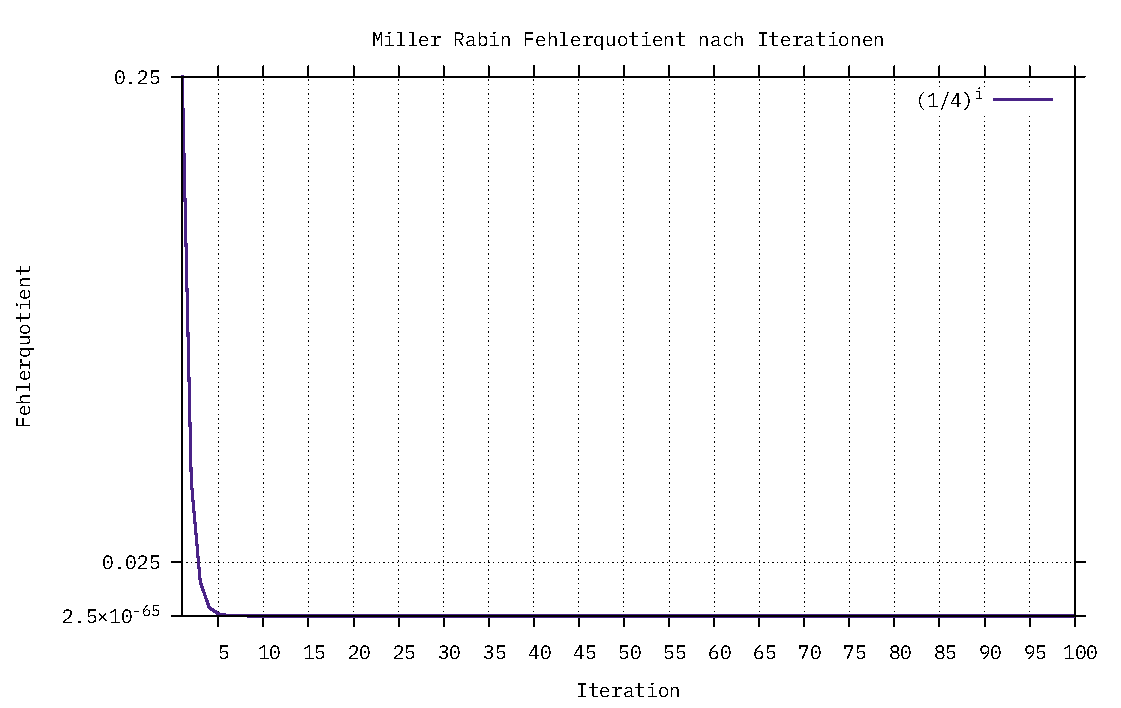
\includegraphics{mr_error.pdf}
  \label{mr_error}
  \caption{Fehlerquotient für $\left\{\,i \in \mathbb{N}\mid 1 \le i \le 100 \, \right\}$}
\end{figure}

\newpage

\subsubsection{Fermatscher Primzahltest}

Der kleine fermatsche Satz kann als rudimentärer Primzahltest verwendet werden, da die Kongruenz zwischen $a$ und $p$ nur gegeben ist, wenn $p$ eine Primzahl ist. Somit kann durch das iterative Testen dieser Kongruenz mit verschiedenen Basen $a$ ein Schluss auf die Primalität von $p$ gezogen werden:

\begin{figure}[h]
  \begin{cminted}

  // Falls die zu überprüfende Zahl 3 oder 2 ist
  if (n == 3 || n == 2)
    // Wahr zurückgeben
    return true;

  // Führe den Primzahltest für k Iterationen aus, beziehungsweise bis er fehlschlägt
  for (int _ = 0; _ < k; _++)
  {

    // Label zu dem gesprungen wird falls keine teilerfremde Base a gefunden werden konnte
    Restart:
                
    // Zufällige Base a mit 2 ≤ a ≤ n-2
    BigInteger a = GetRandomBigIntInRange(n.GetByteCount(), 2, n - 2);

    // Zählt die Anzahl der Versuche eine teilerfremde Base a basierend auf der selben Zufallszahl zu finden
    int coprimeRuns = 0;

    // Label zu dem gesprungen wird falls die derzeitige Base a nicht teilerfremd ist
    NotCoprime:

    // Falls die Base a mehr als 5 mal nicht teilerfremd war wird eine neue Zufallszahl generiert
    if (coprimeRuns > 5)
      goto Restart;

    // Untersuche ob a und n teilerfremd sind
    if (BigInteger.GreatestCommonDivisor(a, n) != 1)
    {
      // erhöhe die Base a um eins
      a++;
      // erhöhe die Anzahl der Versuche um eins
      coprimeRuns++;
      // springe zum vorherigen Label
      goto NotCoprime;
    }

    // Berechne a^n-1 mod n
    BigInteger res = ModPow(a, n - 1, n);

    // Falls der Rest nicht eins ist ist n nicht prim
    if (res != 1)
    {
      // Gebe falsch zurück
      return false;
    }
  }
  \end{cminted}
  \caption{Implementation eines Primzahltestes basierend auf dem kleinen fermatschen Satz}
\end{figure}

\newpage

\section{Eulersche Phi-Funktion}
\newpage

\section{Carmichael-Funktion}
\newpage

\section{Euklidischer Algorithmus}
\newpage

\subsection{Erweiterter Euklidischer Algorithmus}
\newpage

\section{Hamming-Gewicht}
\newpage

\section{Chinesischer Restsatz}

  \newpage
  \chapter{Anwendungsbeispiel}

\section{Schlüsselerzeugung}

\section{Voraussetzungen}

Für die Erzeugung eines Schlüsselpaares werden zwei zufällige große Primzahlen $p$ und $q$ so gewählt, dass eine Fastprimzahl $n=pq$ berechnet werden kann. Im Verlauf dieser Arbeit wird immer angenommen, dass $p$ und $q$ die selbe Bitgröße besitzen $pbit=qbit$, wobei dies für den RSA-Algorithmus nicht zwingend notwendig ist.
Um das Errechnen von $p$ und $q$ durch Faktorisierung von $n$ zu Erschweren sollten Primzahlen für $p$ und $q$ gewählt werden, welche beide \textquote{groß}\footnote{Derzeitig sichere RSA-Schlüssel besitzen normalerweise zwischen $1024$- und $4096$-bit} und \textquote{weit} auseinander liegen.
Beide Primfaktoren $p$ und $q$ sind durch die Bitgröße von $n$, für welche in der Regel eine Zweierpotenz gewählt wird, beschränkt, wobei $pbit$ und $qbit$ in der Regel entweder gleich groß oder annähernd gleich groß sind. $pbit$ und $qbit$ seien für jeden Wert $p$ und $q$ als die Bitgröße dieser definiert.
Für $p\ge2$ sei $q\ge3 \land q\ne2$ und für $p\ge3$ sei $q\ge2 \land q\ne3$, da dies die kleinsten Primzahlen sind für welche ein $n$ berechnet werden kann:
\begin{equation}
  \begin{split}
    &\left\{\,p \in \mathbb{P}\mid (q=2 \implies 3 \le p) \oplus (q=3 \implies (2 \le p \land p \ne 3))\, \right\}\\
    &\left\{\,q \in \mathbb{P}\mid (p=2 \implies 3 \le q) \oplus (p=3 \implies (2 \le q \land q \ne 3))\, \right\}\\
    &\left\{\,pbit \in \mathbb{N}\mid 2 \le pbit\, \right\}\\
    &\left\{\,qbit \in \mathbb{N}\mid 2 \le qbit\, \right\}\\
    &pbit=\left\lfloor\frac{\ln{p}}{\ln{2}}\right\rfloor+1=\left\lfloor\log_2{p}\right\rfloor+1\\
    &qbit=\left\lfloor\frac{\ln{q}}{\ln{2}}\right\rfloor+1=\left\lfloor\log_2{q}\right\rfloor+1
  \end{split}
\end{equation}

Somit sei für eine Zahl $p\coloneq2^{2048}-1$ die Bitgröße $pbit$ dementsprechend:

\begin{equation}
  pbit=\left\lfloor\log_2{p}\right\rfloor+1=2048
\end{equation}

Folgend sei für jeden Wert $n$ die Bitgröße $nbit$:

\begin{equation}
  \begin{split}
    &\left\{\,nbit \in \mathbb{N}\mid 3 \le nbit\, \right\}\\
    &nbit=\left\lfloor\frac{\ln{n}}{\ln{2}}\right\rfloor+1=\left\lfloor\log_2{n}\right\rfloor+1\\
    &nbit=pbit+qbit
  \end{split}
\end{equation}

Somit ergibt sich für $nbit\coloneq4096$, $pbit\coloneq2048$ und $qbit\coloneq2048$:

\begin{equation}
  \left\{\,n \in \mathbb{P} \times \mathbb{P}\mid n \ne 4 \land 6 \le n \le 2^{4096}-1\, \right\}
\end{equation}
\newpage
Zwischen 1991 und 2007 veröffentlichte RSA Laboratories die sogenannten \textquote{RSA-Zahlen}. Diese Zahlen waren verschiedene Werte $n$ zwischen 100- und 2048-bit. Ziel dieser Aktion war es die Forschung im Bereich der effizienten Faktorisierung voranzutreiben, dies wurde durch beträchtliche Preisgelder für einige dieser Zahlen bezweckt. Zum derzeitigem Standpunkt ist \textquote{RSA-250} die zuletzt Faktorisierte \textquote{RSA-Zahl} mit 829-bit\cite{rsa250}. Die nächste \textquote{RSA-Zahl} \textquote{RSA-260} enthält $862$-bit und wurde bis zu diesem Zeitpunkt nicht faktorisiert. Somit ergeben sich für $p$, $q$, $n$ und $nbit$ durch die Primfaktoren von \textquote{RSA-250} neue Mindestanforderungen:
\begin{equation}
  \begin{split}
    a&=641352894770715802787901901705773890848250147429434472081168596\\\hookrightarrow&\phantom{=}\;\,32024532344630238623598752668347708737661925585694639798853367\\
    b&=333720275949781565562260106053551142279407603447675546667845209\\\hookrightarrow&\phantom{=}\;\,87023841729210037080257448673296881877565718986258036932062711\\
    &\left\{\,p \in \mathbb{P}\mid (p=a \implies a \le p \land b \le q) \oplus (p=b \implies b \le p \land a \le q)\, \right\}\\
    &\left\{\,q \in \mathbb{P}\mid (q=a \implies a \le q \land b \le p) \oplus (q=b \implies b \le q \land a \le p)\, \right\}\\
    &\left\{\,n \in \mathbb{P} \times \mathbb{P}\mid 2^{862}-1 < n\, \right\}\\
    &\left\{\,nbit \in \mathbb{N}\mid 862 < nbit\, \right\}
  \end{split}
\end{equation}

Das Bundesamt für Sicherheit in der Informationstechnik empfiehlt die Verwendung von RSA-Schlüsseln mit mehr als 3000-bit, um sicherzustellen, dass der Modulus $n$ derzeit nicht faktorisiert werden kann.\cite{bsicrypto} Somit ergeben sich erneut neue Definitionen für $p$, $q$, $n$, $pbit$, $qbit$ und $nbit$:

\begin{equation}
  \begin{split}
    &\left\{\,p \in \mathbb{P}\mid 2^{1500}-1 \le p\, \right\}\\
    &\left\{\,q \in \mathbb{P}\mid 2^{1500}-1 \le q\, \right\}\\
    &\left\{\,n \in \mathbb{P} \times \mathbb{P}\mid 2^{3000}-1 \le n\, \right\}\\
    &pbit=\left\lfloor\frac{\ln{p}}{\ln{2}}\right\rfloor+1=\left\lfloor\log_2{p}\right\rfloor+1=1500\\
    &qbit=\left\lfloor\frac{\ln{q}}{\ln{2}}\right\rfloor+1=\left\lfloor\log_2{q}\right\rfloor+1=1500\\
    &nbit=\left\lfloor\frac{\ln{n}}{\ln{2}}\right\rfloor+1=\left\lfloor\log_2{n}\right\rfloor+1=3000\\
    &nbit=pbit+qbit\\
    &n=p\cdot q
  \end{split}
\end{equation}
\newpage

Als Teil meiner Arbeit werde ich $nbit=4096$ als Bitgröße verwenden, da $4096$-Bit die derzeit größte weit verbreitete Schlüsselgröße bei RSA-Schlüsseln ist. Im Weiteren werde ich davon ausgehen, dass $p$ und $q$ die selbe Bitröße besitzen. Somit ergeben sich für diese Arbeit folgende finale Definitionen für $p$, $q$, $n$, $pbit$, $qbit$ und $nbit$:
\begin{equation}
  \begin{split}
    &\left\{\,p \in \mathbb{P}\mid p \le 2^{2048}-1\, \right\}\\
    &\left\{\,q \in \mathbb{P}\mid p \le 2^{2048}-1\, \right\}\\
    &\left\{\,p \in \mathbb{P}\mid (p=2 \implies (2 \le p \le 2^{2048}-1 \land p \ne 3) \land (3 \le q \le 2^{2048}-1))\, \oplus \right. \\ &\hookrightarrow \left. (p=3 \implies (3 \le p \le 2^{2048}-1) \land (2 \le q \le 2^{2048}-1 \land q \ne 3))\, \right\}\\
    &\left\{\,q \in \mathbb{P}\mid (q=2 \implies (2 \le q \le 2^{2048}-1 \land q \ne 3) \land (3 \le p \le 2^{2048}-1)\, \oplus \right. \\ &\hookrightarrow \left. (q=3 \implies (3 \le q \le 2^{2048}-1) \land (2 \le p \le 2^{2048}-1 \land p \ne 3)\, \right\}\\
    &\left\{\,n \in \mathbb{P} \times \mathbb{P}\mid n \le 2^{4096}-1\, \right\}\\
    &pbit=2048\\
    &qbit=2048\\
    &nbit=4096\\
  \end{split}
\end{equation}


\newpage
\section{Schlüsselverteilung}
\newpage
\section{Verschlüsselung}
\newpage
\section{Entschlüsselung}
\newpage
\section{Signatur}

  \newpage
  \chapter{Auswertung}

\section{Faktorisierung von \textquote{RSA-155}}

Als Teil meiner Arbeit und als Demonstration der Nötigkeit von immer größeren Bitgrößen für $n$ habe ich unter Verwendung der \textquote{\href{https://cado-nfs.gitlabpages.inria.fr/}{CADO-NFS}} Software, welche eine Implementation des \textquote{\textbf{N}umber \textbf{F}ield \textbf{Sieve}}-Algorithmuses (Zahlkörpersiebalgorithmus) bereitstellt eine Primfaktorzerlegung vorgenommen. Für Zahlen größer als $10^{100}$ ist der Zahlkörpersieb der effizienteste bekannte Algorithmus zur Primfaktorzerlegung\cite{SO2267146}. \textquote{RSA-155} ist eine Fastprimzahl mit $512$-bit und somit größer als $10^{100}$, welche 1999 von einem Team unter der Leitung von Herman te Riele in acht Monaten faktorisiert wurde\cite{rsa155}. Fünfundzwanzig Jahre später war ich in der Lage \textquote{RSA-155} auf einem Intel Pentium G4400T aus dem Jahre 2015 in nur rund zwanzig Tagen\footnote{$1.77025 \times 10^{6}$ Sekunden entsprechen 20 Tagen 11 Stunden 44 Minuten und 08 Sekunden} zu faktorisieren. Dies zeigt klar, dass die Faktorisierung von Fastprimzahlen im Laufe der Zeit durch Fortschritte im Bereich der Primfaktorzerlegung und einen breiteren öffentlichen Zugang zu Leistungsstarken Computern und entsprechenden Softwarepaketen um einiges erleichtert wurde. Dadurch werden größere Werte $n$ zwingend nötig, da RSA-Schlüssel sonst in für einen Angreifer realisierbarer Zeit gebrochen werden könnten. Angreifer mit ausreichenden Rechenresourcen, wie zum Beispiel staatlich unterstützte Akteure oder solche mit Cloud- oder Clustercomputern können RSA-Schlüssel mit solch geringer Bitgröße in einer noch kürzeren Zeit brechen. Meine Faktorisierung hat die erwarteten Primfaktoren $106603488380168454820927220360012878679207958575989291522270608237193062808643$ und $102639592829741105772054196573991675900716567808038066803341933521790711307779$ geliefert, welche auch 1999 so errechnet wurden:

\begin{equation}
  \begin{split}
    p&=106603488380168454820927220360012878679207958575989291522270608237193062808643\\
    q&=102639592829741105772054196573991675900716567808038066803341933521790711307779\\
    n&=pq=1094173864157052742180970732204035761200373294544920599091384213147634998\\\hookrightarrow&\phantom{=}\;\,4288934784717997257891267332497625752899781833797076537244027146743531593354333897
  \end{split}
\end{equation}

% [32;1mInfo[0m:Complete Factorization / Discrete logarithm: Total cpu/elapsed time for entire Complete Factorization 3.22105e+06/1.77025e+06 [20d 11:44:08]

% 1770250.00000 / 86400
% 20.489004629629629629629629629629629629629629629629629629629629629629629629629629629629629629629629629629629629629629629629629629629629629629629629629629629629629629629629629629629629629629629629629629629629629629629629629629629629629629629629629629629629629629629629629629629629629629629629629629629629

% 106603488380168454820927220360012878679207958575989291522270608237193062808643 102639592829741105772054196573991675900716567808038066803341933521790711307779

\newpage

\section{Selbstständigkeitserklärung}

Hiermit erkläre ich, dass ich die vorliegende Arbeit mit dem Titel \textquote{Bedeutung von starken Primzahlen — Eine Einführung in das RSA-Verschlüsselungssystem} selbstständig und ohne unerlaubte fremde Hilfe angefertigt, keine anderen als die angegebenen Quellen und Hilfsmittel verwendet und die den verwendeten Quellen und Hilfsmitteln wörtlich oder inhaltlich entnommenen Stellen als solche kenntlich gemacht habe.
\vspace{4em}

\hrule width25em
\vspace{0.5em}
Ort, Datum\hspace{11.5em} Unterschrift

  \newpage
  \backmatter{}

  \nocite{*}
  \printbibliography{}
\end{document}
